\documentclass{article}

% Language setting
% Replace `english' with e.g. `spanish' to change the document language
\usepackage[english]{babel}
\usepackage{multicol}
\usepackage{listings}
\usepackage{tikz}

% Set page size and margins
% Replace `letterpaper' with `a4paper' for UK/EU standard size
\usepackage[letterpaper,top=2cm,bottom=2cm,left=3cm,right=3cm,marginparwidth=1.75cm]{geometry}
\usepackage{amsfonts} 

% Useful packages
\usepackage{amsmath}
\usepackage{graphicx}
\usepackage[colorlinks=true, allcolors=blue]{hyperref}

% laisser la premiere page vide, seulement le titre du projet
% mettre la page avec les noms en deuxieme
% mettre la troisieme page comme le truc ou y a quoi dans chaque page
% mettre la quatrieme page en vide
% start les pages

\graphicspath{ {./} }

\title{Compte Rendu Projet THL}

\author{
  Kichou, Nadir\\
  \texttt{nadirkichou@hotmail.fr}
  \and
  Berrada, Serine\\
  \texttt{serineber@outlook.com}
   \and
  Mansoura, Wael\\
  \texttt{wael@gmail.com}
   \and
  Ouldali, Najib\\
  \texttt{najib@gmail.com}
  \and
  Seddiki, Yacine\\
  \texttt{yacine@gmail.com}
}

\begin{document}

\maketitle

\pagebreak

\setcounter{tocdepth}{1} % Show sections

\tableofcontents

\pagebreak

\section{Automate Choisi}

Nous avons choisi un automate pour reconnaitre tout les nombres dans $\mathbb{R}$ $$1, 2.0, -4.5, 10, +10, 0.45, -0.78, 85, 10.55 \ldots$$

\section{Descripton de l'Automate Choisi}

\subsection{Definition}

$$A = (\Sigma, E, e_0, F, \Delta)$$\\
Alphabet: $\Sigma = \{0, 1, 2, 3, 4, 5, 6, 7, 8, 9, ., -, +\}$\\
Etats: $E = \{e_0, e_1, e_2, e_3, e_4, e_5\}$\\
Etats Finaux: $F = \{e_2, e_3, e_5\}$\\
Etat Initial: $e_0 = e_0$\\
Transitions:
\begin{multicols}{2}
\begin{itemize}
  \item \tab $\delta(e_0, +) = e_1$
  \item \tab $\delta(e_0, -) = e_1$
  \item \tab $\delta(e_0, 0) = e_2$
  \item \tab $\delta(e_0, 1) = e_3$
  \item \tab $\delta(e_0, 2) = e_3$
  \item \tab $\ldots$
\end{itemize}
\end{multicols}

\subsection{Representation Matricielle}
  \begin{tabular}{| c | c | c | c | c | c | c | c | c | c | c | c | c | c |}
    \hline
    State & 0 & 1 & 2 & 3 & 4 & 5 & 6 & 7 & 8 & 9 & . & - & + \\
    \hline
    $e_0$ & $e_2$ & $e_3$ & $e_3$ & $e_3$ & $e_3$ & $e_3$ & $e_3$ & $e_3$ & $e_3$ & $e_3$ & $e_p$ & $e_1$ & $e_1$ \\
    \hline
    $e_1$ & $e_2$ & $e_3$ & $e_3$ & $e_3$ & $e_3$ & $e_3$ & $e_3$ & $e_3$ & $e_3$ & $e_3$ & $e_p$ & $e_p$ & $e_p$ \\
    \hline
    $e_2$ & $e_p$ & $e_p$ & $e_p$ & $e_p$ & $e_p$ & $e_p$ & $e_p$ & $e_p$ & $e_p$ & $e_p$ & $e_4$ & $e_p$ & $e_p$ \\
    \hline
    $e_3$ & $e_3$ & $e_3$ & $e_3$ & $e_3$ & $e_3$ & $e_3$ & $e_3$ & $e_3$ & $e_3$ & $e_3$ & $e_4$ & $e_p$ & $e_p$ \\
    \hline
    $e_4$ & $e_5 & $e_5 & $e_5 & $e_5 & $e_5 & $e_5 & $e_5 & $e_5 & $e_5 & $e_5 & $e_p$ & $e_p$ & $e_p$ \\
    \hline
    $e_5$ & $e_5$ & $e_5$ & $e_5$ & $e_5$ & $e_5$ & $e_5$ & $e_5$ & $e_5$ & $e_5$ & $e_5$ & $e_p$ & $e_p$ & $e_p$ \\
    \hline
\end{tabular}

\subsection{Representation Graphique}


\begin{center}
  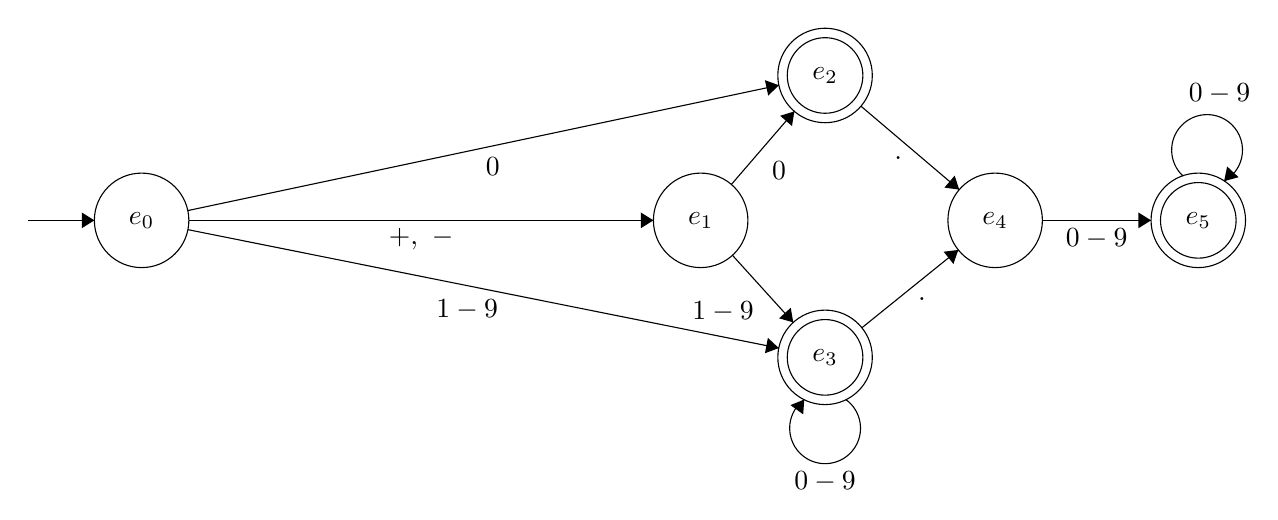
\begin{tikzpicture}[scale=0.2]
  \tikzstyle{every node}+=[inner sep=0pt]
  \draw [black] (44.1,-27.1) circle (3);
  \draw (44.1,-27.1) node {$e_1$};
  \draw [black] (52,-35.8) circle (3);
  \draw (52,-35.8) node {$e_3$};
  \draw [black] (52,-35.8) circle (2.4);
  \draw [black] (52,-17.9) circle (3);
  \draw (52,-17.9) node {$e_2$};
  \draw [black] (52,-17.9) circle (2.4);
  \draw [black] (62.8,-27.1) circle (3);
  \draw (62.8,-27.1) node {$e_4$};
  \draw [black] (8.6,-27.1) circle (3);
  \draw (8.6,-27.1) node {$e_0$};
  \draw [black] (75.7,-27.1) circle (3);
  \draw (75.7,-27.1) node {$e_5$};
  \draw [black] (75.7,-27.1) circle (2.4);
  \draw [black] (46.12,-29.32) -- (49.98,-33.58);
  \fill [black] (49.98,-33.58) -- (49.82,-32.65) -- (49.08,-33.32);
  \draw (47.51,-32.91) node [left] {$1-9$};
  \draw [black] (53.323,-38.48) arc (54:-234:2.25);
  \draw (52,-43.05) node [below] {$0-9$};
  \fill [black] (50.68,-38.48) -- (49.8,-38.83) -- (50.61,-39.42);
  \draw [black] (46.05,-24.82) -- (50.05,-20.18);
  \fill [black] (50.05,-20.18) -- (49.15,-20.46) -- (49.9,-21.11);
  \draw (48.6,-23.95) node [right] {$0$};
  \draw [black] (54.28,-19.85) -- (60.52,-25.15);
  \fill [black] (60.52,-25.15) -- (60.23,-24.26) -- (59.58,-25.02);
  \draw (56.64,-22.99) node [below] {$.$};
  \draw [black] (54.34,-33.92) -- (60.46,-28.98);
  \fill [black] (60.46,-28.98) -- (59.53,-29.09) -- (60.15,-29.87);
  \draw (58.16,-31.94) node [below] {$.$};
  \draw [black] (11.6,-27.1) -- (41.1,-27.1);
  \fill [black] (41.1,-27.1) -- (40.3,-26.6) -- (40.3,-27.6);
  \draw (26.35,-27.6) node [below] {$+,\mbox{ }-$};
  \draw [black] (1.4,-27.1) -- (5.6,-27.1);
  \fill [black] (5.6,-27.1) -- (4.8,-26.6) -- (4.8,-27.6);
  \draw [black] (11.53,-26.48) -- (49.07,-18.52);
  \fill [black] (49.07,-18.52) -- (48.18,-18.2) -- (48.39,-19.18);
  \draw (30.9,-23.08) node [below] {$0$};
  \draw [black] (11.54,-27.69) -- (49.06,-35.21);
  \fill [black] (49.06,-35.21) -- (48.37,-34.56) -- (48.18,-35.54);
  \draw (29.27,-32.11) node [below] {$1-9$};
  \draw [black] (65.8,-27.1) -- (72.7,-27.1);
  \fill [black] (72.7,-27.1) -- (71.9,-26.6) -- (71.9,-27.6);
  \draw (69.25,-27.6) node [below] {$0-9$};
  \draw [black] (74.72,-24.277) arc (226.87498:-61.12502:2.25);
  \draw (77.05,-19.74) node [above] {$0-9$};
  \fill [black] (77.34,-24.61) -- (78.26,-24.36) -- (77.53,-23.68);
  \end{tikzpicture}
\end{center}

\section{Fichier D'Entré}
Le fichier d'entré est sous cette forme

\definecolor{codegreen}{rgb}{0,0.6,0}
\definecolor{codegray}{rgb}{0.5,0.5,0.5}
\definecolor{codepurple}{rgb}{0.58,0,0.82}
\definecolor{backcolour}{rgb}{0.95,0.95,0.92}

\lstdefinestyle{mystyle}{
    backgroundcolor=\color{backcolour},   
    commentstyle=\color{codegreen},
    keywordstyle=\color{magenta},
    numberstyle=\tiny\color{codegray},
    stringstyle=\color{codepurple},
    basicstyle=\ttfamily\footnotesize,
    breakatwhitespace=false,         
    breaklines=true,                 
    captionpos=b,                    
    keepspaces=true,                 
    numbers=left,                    
    numbersep=5pt,                  
    showspaces=false,                
    showstringspaces=false,
    showtabs=false,                  
    tabsize=2
}

\lstset{style=mystyle}

\lstinputlisting[language=Octave]{file.txt}

\section{Structures de Données}
Pour stocker les noms des etats et les identifier nous avons utilisé des entiers au lieu de chaines de characteres pour un soucis de simplicité\\

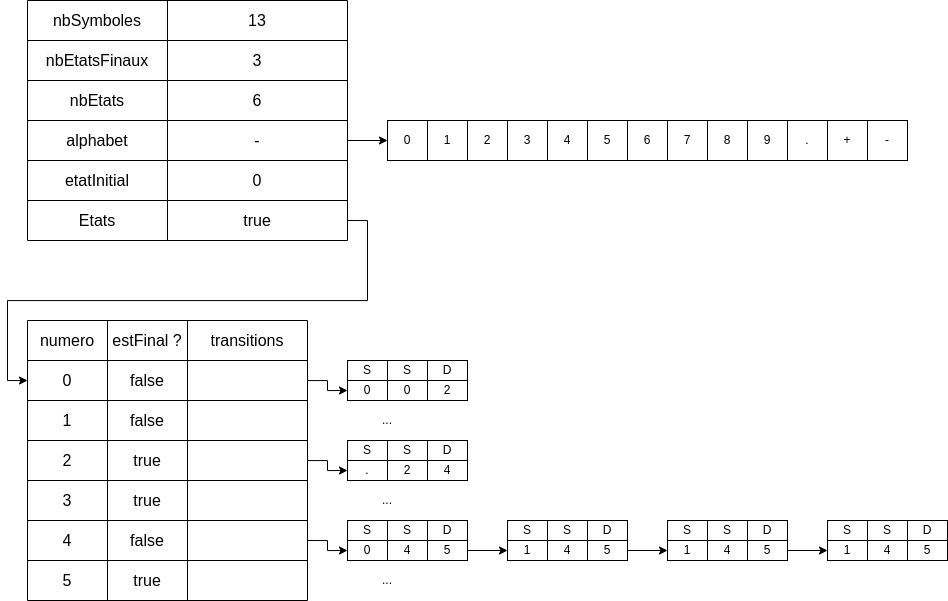
\includegraphics[width=\textwidth]{diagramme.png}\\

\begin{lstlisting}[language=C, caption=Structure Automate]
{
  int nbSymboles;
  int nbEtats;
  int nbEtatsFinaux;
  char *alphabet;
  // TODO: change to string ?
  int etatInitial;
  Etat **etats;
};
\end{lstlisting}

\begin{lstlisting}[language=C, caption=Structure Etat]
struct Etat
{
  // TODO: change to string
  int numero;
  bool estFinal;
  List *transitions;
};
\end{lstlisting}

\begin{lstlisting}[language=C, caption=Structure Etat]
struct Transition
  {
  char symbole;
  // TODO: change to string
  int source;
  // TODO: change to string
  int destination;
};
\end{lstlisting}



\section{Captures D'Ecran de L'execution}

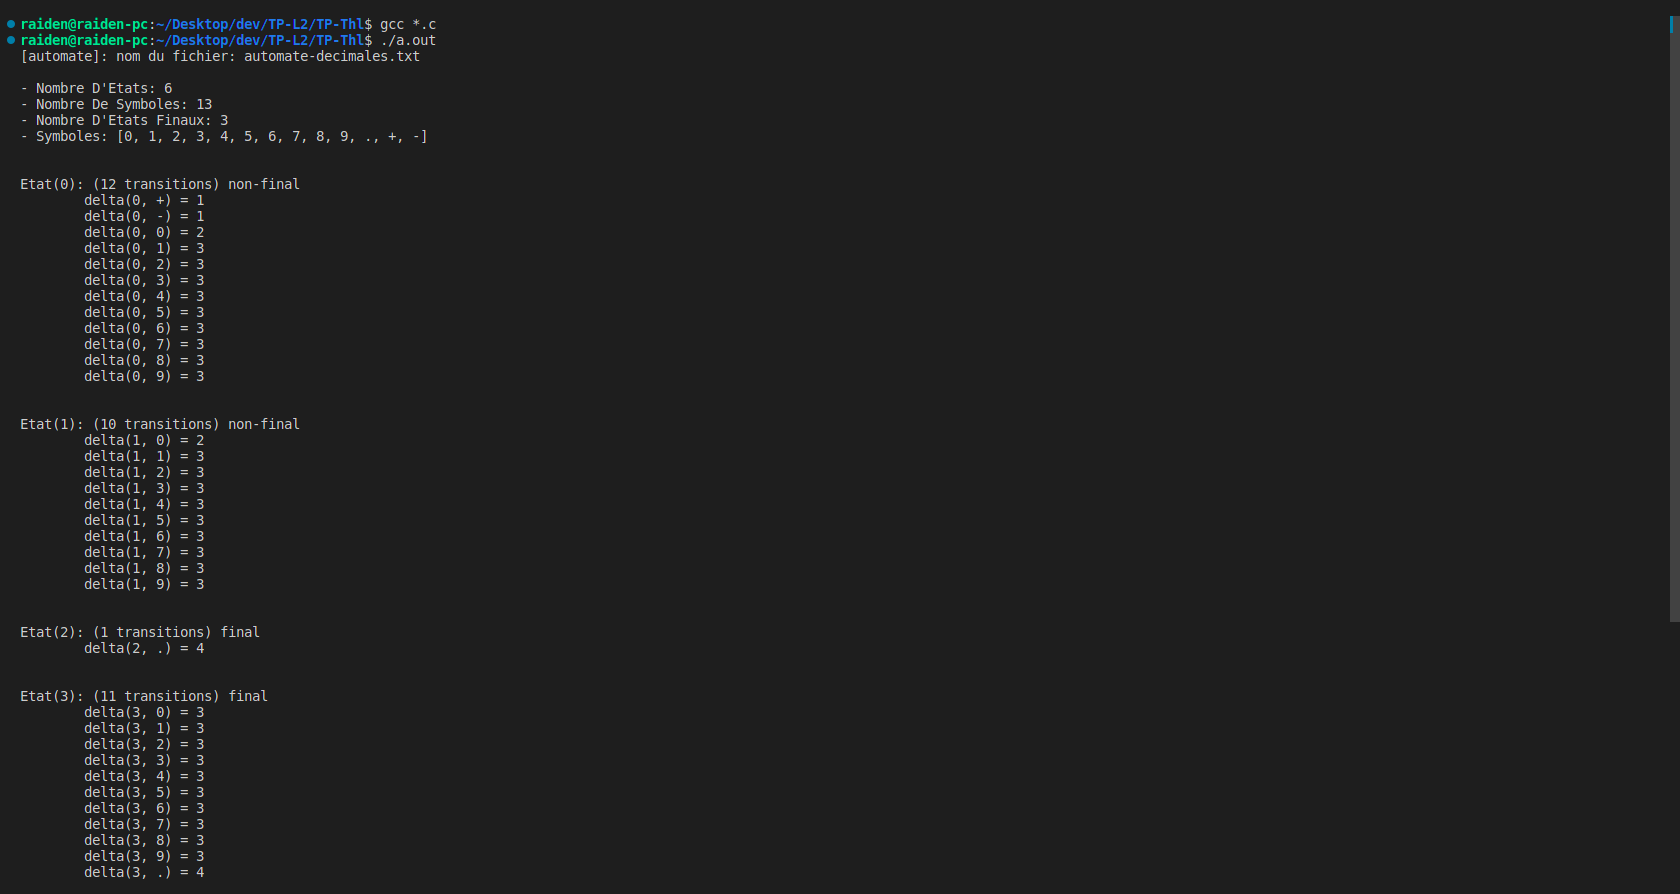
\includegraphics[width=\textwidth]{screen-1.png}
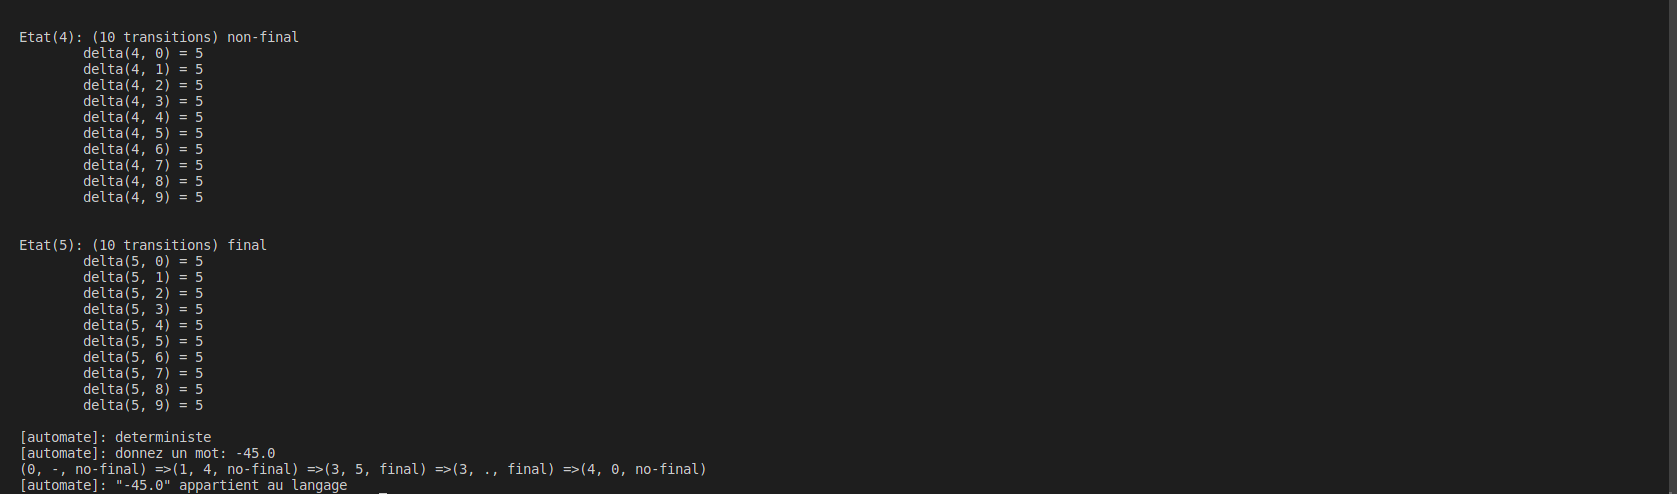
\includegraphics[width=\textwidth]{screen-2.png}

\section{Autre}

Si vous souhaitez consulter le code du projet vous pourrez le retrouver sur mon \href{https://www.github.com/raideno/projet}{github}.

\end{document}